\chapter{Problemanalyse}
    \label{chapter:ProblemAnalysis}
    \section{\imperia}
        \subsection{Dokumente}
        \subsection{Vorlagen}
        \subsection{Workflows}
        \subsection{Architektur}
            \begin{figure}[hbt]
                \centering
                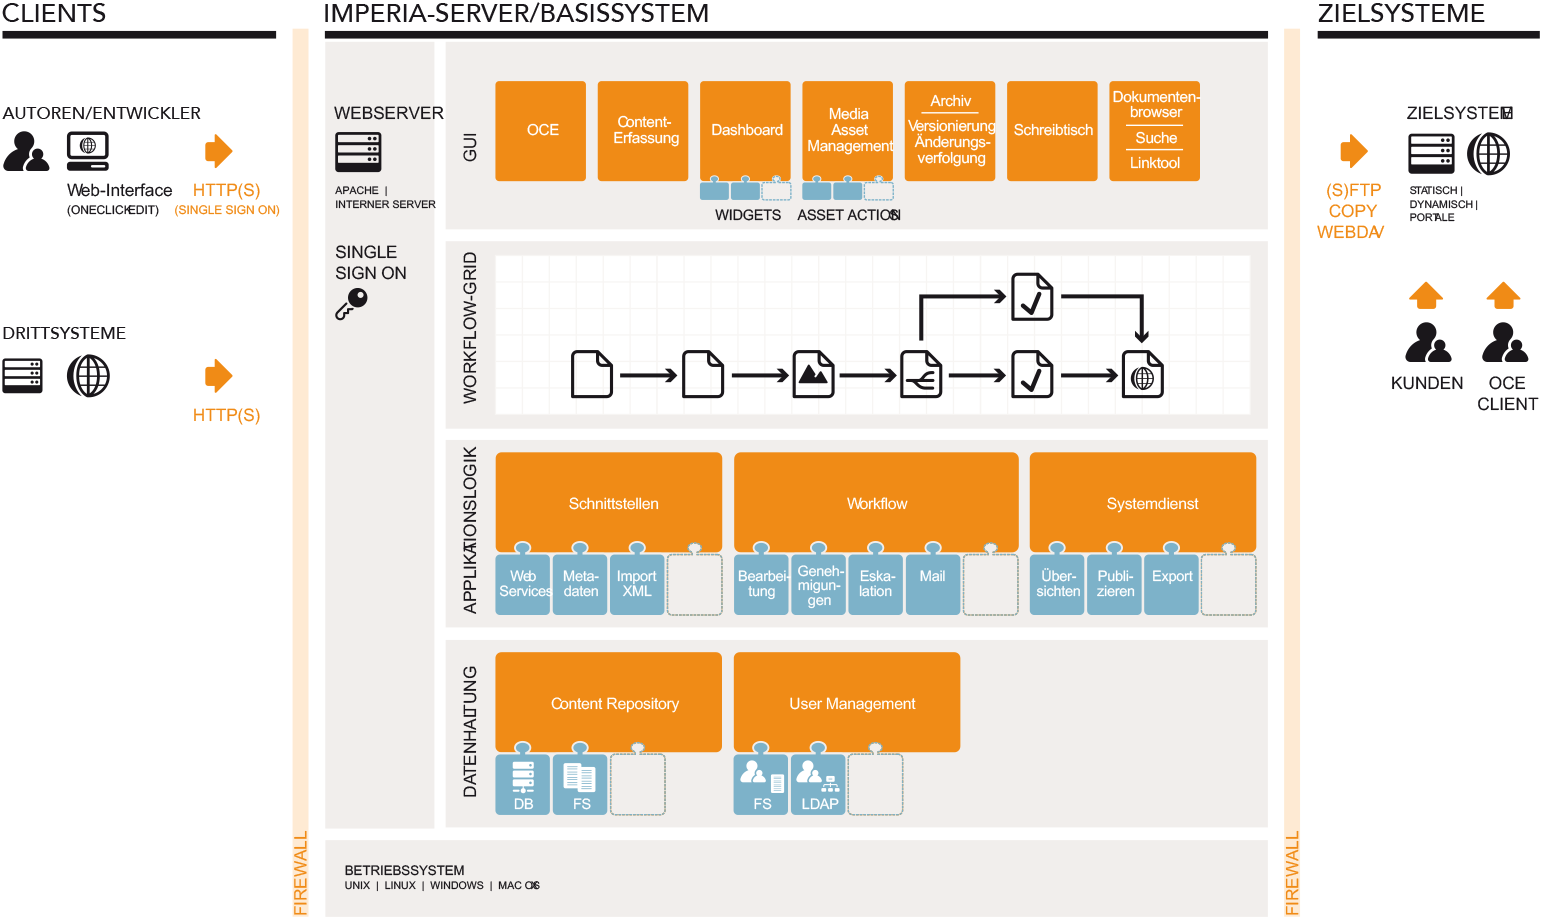
\includegraphics[width=\textwidth]{../resources/imperia/architektur.png}
                \caption{Architkektur von {\imperia} \cite{imperia:ecmd}}
                \label{image:imperiaArchitektur}
            \end{figure}

    \section{\wordpress}
        \subsection{Posts und Pages}
        \subsection{Vorlagen und Themes}
        \subsection{Plugins}

    \section{Klassifizierung der Inhalte einer Webseite}
        %\url{http://www.fernuni-hagen.de/KSW/portale/babw/service/}

        %\begin{figure}
        %    \centering
        %    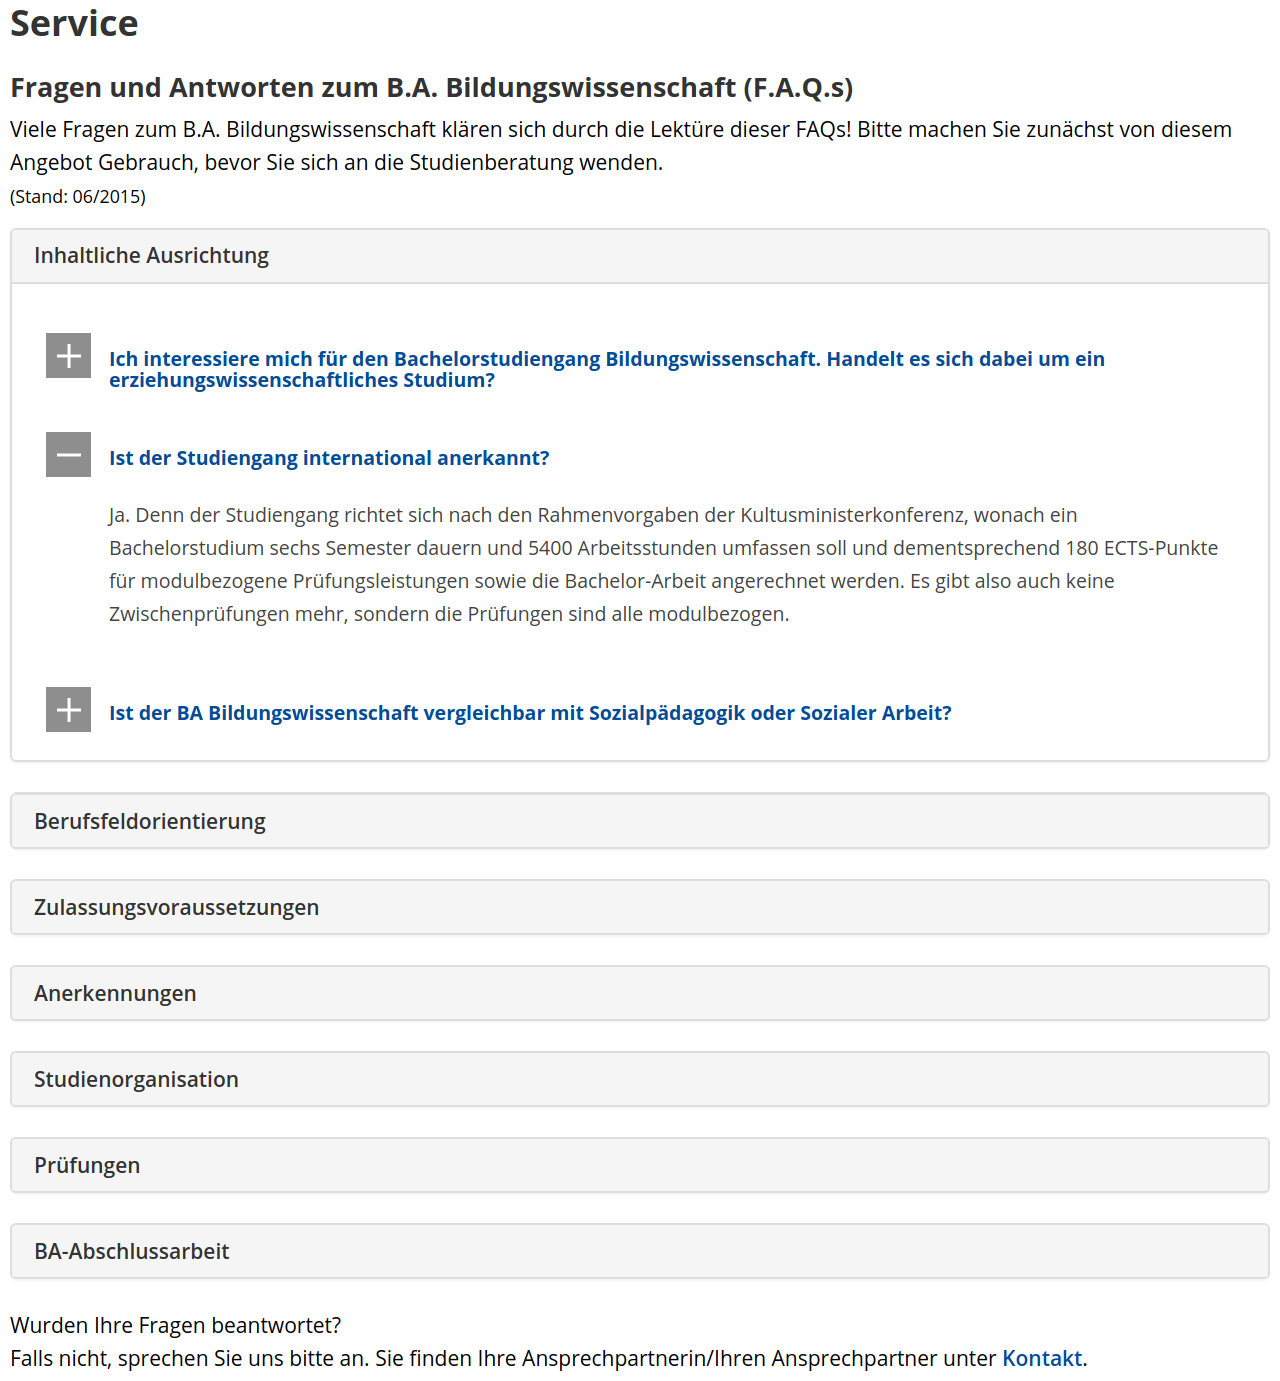
\includegraphics[width=\textwidth]{../resources/babw_service_faq.png}
        %    \caption{FAQ Seite des Studienportals B.A. Bildungswissenschaft}
        %    \label{image:BuildingBlocks}
        %\end{figure}
    
    \section{Das World Wide Web}
        \label{section:TheWWW}
        % TODO Keine umfassende Betrachtung, da zu viel. Nur Aspekte, die für Arbeit wichtig.
        Zur Lösung der beschriebenen Problemstellung ist eine genauere
        Betrachtung ihrer Domäne notwendig.
        Das Problem wird dadurch in einen größeren Kontext gesetzt,
        was zu einem besseren Verständnis und damit zur Findung
        einer geeigneten Lösung beiträgt.
        % TODO: Ref auf DDD?

        Die in diesem Fall zu betrachtende Domäne ist das "`\gls{www}"'.
        Diese wird im Folgenden aus zwei Perspektiven betrachtet:
        Zunächst wird die Sicht eines Webseitenbesuchers auf das \gls{www} beschrieben.
        Anschließend stehen die konzeptionellen und technischen Grundlagen
        des \gls{www} im Vordergrund.
        Zusammen vermitteln diese Erläuterungen hinreichendes Wissen,
        um eine Lösung für die gegebene Problemstellung zu erarbeiten.

        \subsection{Das World Wide Web für Webseitenbesucher}
            \label{section:enduserViewOnWWW}
            Die Sicht eines Webseitenbesuchers (im Folgenden auch "`Endnutzer"' genannt)
            auf das \gls{www} ist simpel und sollte von jedem Leser nachvollzogen werden können.
            Dennoch bietet sie wichtige Einblicke.

            \paragraph*{Der Browser}
            Zugang zum \gls{www} erhält ein typischer Endnutzer über einen \textit{Browser}.
            In dessen Adresszeile trägt er einen \gls{url} ein,
            woraufhin der Browser die gewünschte Webseite lädt und anzeigt.
            Eine Webseite ist aus Sicht eines Endnutzers also eindeutig über eine
            Adresse, die allgemein "`URL"' oder "`Link"' genannt wird, gekennzeichnet.
            Der Browser dient zur Anzeige von Webseiten, wodurch er für Webseitenbesucher
            zu einem unentbehrlichen Werkzeug wird.
            Browser existieren für verschiedene Endgeräte,
            wie PCs, Smartphones und Tablets.
            Das heißt ein Webseitenbesucher ist nicht an eine Form von Endgeräten gebunden.

            \paragraph*{Bestandteile}
            Sieht sich ein Besucher eine Webseite im Browser an,
            kann er schnell verschiedene Bestandteile ausmachen.
            Dazu zählen zunächst simple Elemente, mit denen er wenig bis gar nicht
            interagieren kann, also statischer Natur sind.
            Vertreter dieser Gruppe sind

            \begin{itemize}
                \item Texte,
                \item Bilder,
                \item Videos,
                \item Links auf andere Webseiten und
                \item Dateien, die zum Download bereitstehen.
            \end{itemize}

            Des Weiteren besitzt eine Webseite Designelemente,
            die in ihrem Aufbau oder ihrer Funktion komplexer
            als die zuvor genannten sind.
            Die Bibliothek Bootstrap\footnote{https://getbootstrap.com/}
            enthält zahlreiche solcher Komponenten.
            Beispielsweise bietet die Komponente "`Card"' die Möglichkeit
            Inhalte in komplexe Behälter einzubetten \cite{bootstrap:Cards}.
            Ein anderes Beispiel ist die Komponente "`Carousel"',
            welche der Erstellung von Diashows dient \cite{bootstrap:Carousel}.
            Letztere und viele weitere bieten dem Nutzer
            erweiterte Möglichkeiten zur Interaktion mit einer Webseite.

            Das gilt auch für Formular- oder Steuerelemente,
            die aus klassischen Applikationen bekannt sind,
            aber auch in Webseiten Anwendung finden.
            Dazu gehören unter anderem

            \begin{itemize}
                \item Textfelder,
                \item Schaltflächen,
                \item Dropdown-Listen,
                \item Checkboxen und
                \item Radiobuttons.
            \end{itemize}

            Allen Elementen ist gemein, dass ihr Aussehen sich von
            zwischen verschiedenen Webseiten unterscheiden kann.

            \paragraph{Varianten}
            Aus Sicht eines Endnutzers existieren oftmals mehrere
            Varianten derselben Webseite.
            Welche Variante er sieht hängt dabei von zwei Dimensionen ab:
            Sprache und Endgerät.

            Die heutige globalisierte und vernetzte Welt machen es oft erforderlich
            einen Internetauftritt auch auf internationele Besucher vorzubereiten.
            An erster Stelle bedeutet dies, dass Inhalte in verschiedene Sprachen
            übersetzt werden, um sie einem möglichst großen Publikum zugänglich zu machen.
            Für einen Endnutzer gibt es prinzipiell zwei Methoden,
            wie er eine Seite in seiner favorisierten Sprache anzeigen kann:

            \begin{itemize}
                \item   Die Webseite bietet ihm ein Steuerelement,
                        über das er selbst eine Sprache auswählen kann.
                \item   Die Webseite ermittelt automatisch die geeignete Sprache,
                        anhand verschiedener Parameter, die für den Besucher nicht zwangsläufig
                        offensichtlich sind.
            \end{itemize}

            Die Popularität mobiler Endgeräte wie Smartphones und Tablets
            bewegt immer mehr Betreiber von Webseiten dazu,
            verschiedene Versionen ihres Internetauftrittes anzubieten,
            die für verschiedene Geräte optimiert sind.
            Aus Sicht eines Besuchers gibt es bis zu drei geräteabhängige
            Varianten einer Webseite. Zwei für die oben genannten mobilen Geräte
            sowie eine weitere für PCs.
            Für ihn sind dabei drei Unterscheidungsmerkmale dieser Varianten offensichtlich:
            Inhalt, Design und Funktionalität.
            Ziel jeder Maßnahme ist es die Anzeigefläche,
            die ein Endgerät bietet, sinnvoll zu nutzen.
            Je kleiner ein Gerät ist, desto geringer ist diese Fläche,
            weshalb Inhalte auf kleineren Geräten weggelassen oder anderes
            dargestellt werden.
            Genauso können gewisse Funktionen einer Webseite nicht gleich
            gut sowohl auf großen PC- als auch auf kleinen Smartphone-Displays
            umgesetzt werden, ohne Anpassungen vorzunehmen.
            
            \paragraph*{Webanwendungen}
            Kapitel \ref{section:ContentManagementAndDesign} hat bereits
            kurz aufgezeigt, wie sich Webseiten stets weiterentwickeln.
            Ein wichtiger Aspekt dieser Weiterentwicklung ist aus Sicht
            eines Webseitenbenutzers, wie stark er mit ihr interagieren kann,
            was schon im Abschnitt über die Bestandteile einer Seite kurz aufgegriffen wurde.

            Angefangen bei simplen Seiten,
            die ursprünglich lediglich dazu gedacht waren Informationen
            bereitzustellen und mit anderen zu
            verlinken \cite{bernersLee:InformationManagement},
            entwickelten sich Webseiten im Laufe der Zeit weiter
            und boten immer mehr Möglichkeiten mit dem Nutzer zu interagieren
            und auf seine Aktionen zu reagieren.
            Folglich hielten immer mehr Merkmale klassischer Computeranwendungen
            Einzug in Webseiten.
            Heute stehen Webseiten klassischen Applikationen in Nichts nach,
            weshalb mit ihnen auch komplexe Anwendungen umgesetzt werden.
            Ein gutes Beispiel hierfür sind Googles Office-Anwendungen
            Docs\footnote{\url{https://www.google.com/intl/de/docs/about/}},
            Sheets\footnote{\url{https://www.google.com/intl/de/sheets/about/}},
            und Slides\footnote{\url{https://www.google.com/intl/de/slides/about/}},
            die in der Lage sind in vielen Fällen klassische Office-Anwendungen zu ersetzen.
            Aufgrund dieses besonderen Charakters ist für solche Webseiten auch der Begriff
            "`Webanwendung"' gebräuchlich.

            Im Vergleich zu herkömmlichen Anwendungen besitzen Webanwendungen zwei wichtige Vorteile.
            Solange man einen Internetzugang hat, sind sie zu jeder Zeit und von jedem Ort aus nutzbar.
            Des Weiteren können sie auf jedem Gerät ausgeführt werden,
            das einen Browser besitzt. Wie zuvor beschrieben ist dies nicht mehr ausschließlich ein PC,
            sondern auch mobile Endgeräte wie Smartphones und Tablets.

            \paragraph*{Websites}
            Der Internetauftritt einer Organisation besteht selten aus einer
            einzelnen Webseite.
            Stattdessen besteht er aus vielen Webseiten,
            die untereinander verlinkt sind und von der jede einen eigenen
            \gls{url} besitzt.
            Neben "`Internetauftritt"' hat sich der Begriff "`Website"' zur
            Referenzierung dieser Gesamtheit aller Webseiten einer Organisation
            etabliert \cite{duden:Internetauftritt, oxford:Website}.

            \paragraph*{Klassifizierung}
            Basierend auf ihrer primären Funktion lassen sich Webseiten grob klassifizieren.
            Die Bezeichnungen der resultierenden Klassen finden sich häufig im Sprachgebrauch
            von Webseitenbesucher wieder.

            Die Seiten \url{https://www.google.de} und \url{https://www.bing.com/}
            werden beispielsweise häufig als \textit{Suchmaschinen} bezeichnet.
            Andere geläufige Klassen sind:

            \begin{itemize}
                \item Online-Shops,
                \item Blogs,
                \item Homepages (Internetauftritt einer Organisation oder Privatperson),
                \item Social Networks
                \item Wikis
            \end{itemize}

            Eine weitere Kategorie sind die bereits erörterten Webanwendungen,
            also Webseiten, die bewusst als Oberflächen vob Anwendungen wahrgenommen werden.

            Viele Webseiten können unterschiedlich klassifiziert werden.
            Jede Suchmaschine und jeder Online-Shop ist gleichzeitig auch eine
            Webanwendung. Wie am Anfang dieses Abschnittes erwähnt ist für die
            Klassifizierung aus Endnutzersicht aber die primäre Funktion einer Webseite
            relevant.

        \subsection{Konzeptionelle und technische Grundlagen}
            Nach der Sicht eines Endnutzers auf das \gls{www},
            folgt in diesem Kapitel eine Erläuterung der Konzepte und Grundlagen,
            auf denen es basiert.

            \paragraph*{Definition des \glspl{w3c}}
            Das \gls{w3c} definiert den Begriff "`World Wide Web"' in \cite{w3c:wwwArch} wie folgt:
    
            \begin{quote}
                The \textit{\textbf{World Wide Web}} (\textit{\textbf{WWW}}, or simply \textit{\textbf{Web}})
                is an information space in which the items of interest, referred to as resources,
                are identified by global identifiers called Uniform Resource Identifiers (\textit{\textbf{URI}}).
            \end{quote}

            Darüber hinaus nennt \cite{w3c:wwwArch} die drei grundlegenden Komponenten des \gls{www}:

            \begin{quote}
                They are identification of resources,
                representation of resource state, and the protocols
                that support the interaction between agents and resources in the space.
            \end{quote}

            \paragraph*{\resources}
            Aus der obigen Definition wird deutlich,
            dass das \gls{www} nicht ausschließlich zur Nutzung von Webseiten
            vorgesehen ist.
            Stattdessen können über das \gls{www} jede Art von {\resources} bezogen werden.
            Neben Webseiten gehören dazu unter anderem auch einfache Textdateien
            und Binärdateien wie zum Beispiel PDFs, Audio- oder Videodateien.

            \paragraph*{Identifizierung von \resources}
            Die Beschreibung des \glspl{w3c} stellt außerdem klar,
            dass {\resources} nicht ausschließlich über \glspl{url} angesprochen werden können.
            Stattdessen geschieht dies über \glspl{uri}, die eine Obermenge von \glspl{url} darstellen
            \cite[Kapitel 1.1.3, Seite 7]{rfc:3986}.
            Jede {\resource} im \gls{www} wird also eindeutig über eine \gls{uri} identifiziert.

            \paragraph*{Interaktion mit dem \gls{www}}
            Wie in Kapitel \ref{section:enduserViewOnWWW} beschrieben ist für Endnutzer
            der Browser das einzige Werkzeug, mit dem sie mit dem \gls{www}
            interagieren können. Wie bereits klargestellt wurde,
            können aus dem \gls{www} allerdings nicht nur Webseiten bezogen werden,
            weshalb es naheliegend ist, dass neben Browsern noch weitere Werkzeuge existieren,
            um {\resources} im \gls{www} anzusprechen.
            Das \gls{w3c} bezeichnet jedes Werkzeug, das dazu in der Lage ist, als
            "`Web agent"' und beschreibt diese Rolle wie folgt:
            "`A person or a piece of software acting on the information
            space on behalf of a person, entity, or process."' \cite[Kapitel 6]{w3c:wwwArch}.
            Eine Spezialisierung stellen die sogenannten "`User agents"' dar,
            die das \gls{w3c} als "`One type of Web agent;
            a piece of software acting on behalf of a person."' beschreibt \cite[Kapitel 6]{w3c:wwwArch}.
            Browser sind User agents, aber zum Beispiel auch Kommandozeilenprogramme
            wie curl\footnote{https://curl.haxx.se/}.
            Ihre persönliche Kennung halten User Agents zum Beispiel im
            HTTP-Header "`User-Agent"' fest \cite[Kapitel 5.5.3, Seite 46]{rfc:7231}.

            Der Prozess, bei dem ein Agent über eine \gls{uri} auf eine {\resource}
            zugreift heißt "`Dereferencing the URI"' \cite[Kapitel 3.1]{w3c:wwwArch}.
            Wie dieser Prozess aussieht hängt von der Funktion des User Agents und der \gls{uri} ab
            \cite[Kapitel 3.1]{w3c:wwwArch}.
            Die Funktion eines User Agents könnte beispielsweise das Abrufen einer
            Repräsentation der {\resource} vorsehen, wohingegen ein anderer Agent
            lediglich prüft, ob eine eben solche Repräsentation existiert.
            Das Schema einer \gls{uri} beschreibt laut Spezifikation
            lediglich, wie die folgende Kennung zu interpretieren ist
            \cite[Kapitel 3.1, Seite 17]{rfc:3986}.
            Viele Schemata sind allerdings nach Protokollen benannt,
            weshalb sie in der Praxis häufig bestimmen,
            wie User Agents auf eine {\resource} zugreifen können
            \cite[Kapitel 3.1]{w3c:wwwArch}.
            
            Schemata, die im \gls{www} häufig Anwendung finden,
            sind zum Beispiel
            http\footnote{\url{https://tools.ietf.org/html/rfc7230\#section-2.7.1}},
            https\footnote{\url{https://tools.ietf.org/html/rfc7230\#section-2.7.2}},
            mailto\footnote{\url{https://tools.ietf.org/html/rfc6068}} und
            data\footnote{\url{https://tools.ietf.org/html/rfc2397}}.
            Für Webseiten sind dabei vor allem http und https
            und die gleichnamigen Protokolle von Bedeutung,
            da \glspl{url} von Webseiten diese vorrangig verwenden.

            Wenn ein Browser oder ein anderer Agent eine Webseite aufruft,
            bedeutet dies allgemein gesprochen, dass der Agent eine Repräsentation
            einer {\resource} anfragt, die er über eine \gls{url} spezifiziert.
            Konkret richtet er diese Anfrage an einen Server,
            wozu er das Protokoll HTTP(S)\footnote{\url{https://tools.ietf.org/html/rfc7231}} und die Methode
            GET\footnote{\url{https://tools.ietf.org/html/rfc7231\#section-4.3.1}} verwendet.

            Falls der Server den \gls{url} der Anfrage auflösen kann,
            antwortet er auf die Anfrage mit der Repräsentation der Webseite,
            die im nächsten Abschnitt behandelt wird.
            Der Browser übernimmt dann das Rendering der Seite und die Ausführung
            von eingebetteten Skripten.

            \paragraph*{Repräsentation einer Webseite}
            Webseiten sind Dokumente, die die Auszeichnungssprache \gls{html} verwenden,
            die aktuell in der Version 5 vorliegt \cite{w3c:html5}.
            Bis zur Version 3.2 war \gls{html} eine Implementierung der Metasprache SGML \cite[Kapitel 3]{w3c:html401}.
            Zusammen mit der Version 4 wurde eine Ausprägung spezifiziert,
            die \gls{html} in eine Implementierung der Sprache XML überführte,
            die den Namen XHTML erhielt \cite{w3c:xhtml}.
            \gls{html}5 definiert eine abstrakte Sprache
            die sowohl mit \gls{html}- als auch mit XML-Syntax genutzt werden kann
            \cite[Kapitel 1.6]{w3c:html5}.
            Einem Agent kann über den MIME-Type mitgeteilt werden,
            ob ein Dokument \gls{html}- oder XML-Syntax verwendet \cite[Kapitel 1.6]{w3c:html5}.
            Diese Angabe ist wichtig, da XML-Syntax restriktiver als \gls{html}-Syntax ist.
            Der \gls{html}-Syntax erfordert zum Beispiel nicht,
            dass alle öffnenden Tags auch einen schließenden Gegenpart besitzen
            \cite[Kapitel 3.2.3]{w3c:html5}.
            
            \gls{html}-Dokumente bestehen in beiden Syntaxvarianten aus verschachtelten
            Nodes, die in 10 Kategorien eingeteilt werden \cite[Kapitel 4]{w3c:html5}.
            Diese sind in Tabelle \ref{table:htmlElements} inkl. einiger Vertreter aufgelistet.

            \begin{table}[h]
                \centering
                \begin{tabular}{|l|l|}
                \hline
                \textbf{Kategorie} & \textbf{Elemente (Auswahl)} \\
                \hline
                Das Wurzelelement & html \\
                \hline
                Metadaten des Dokumentes & head, title, style \\
                \hline
                Absätze & body, article, section \\
                \hline
                Gruppierungen & p, ul, div \\
                \hline
                Semantische Kennzeichnung von Text & a, strong, code \\
                \hline
                Kennzeichnung von Textänderungen & ins, del \\
                \hline
                Eingebetteter Inhalt & img, iframe, object \\
                \hline
                Tabellenelemente & table, tr, td \\
                \hline
                Formulare & form, input, button \\
                \hline
                Skripte & script, canvas \\
                \hline
                \end{tabular}
                \caption{\gls{html} Elemente}
                \label{table:htmlElements}
            \end{table}

            Die verschiedenen Elemente geben ihren Inhalten eine semantische Bedeutung.
            Text in einem h1 Element wird von einem Browser zum Beispiel in die Anzeige gerendert
            \cite[Kapitel 4.3.6]{w3c:html5},
            wohingegen er in einem script Tag als Code interpretiert und ausgeführt wird
            \cite[Kapitel 4.11.1]{w3c:html5}.
            
            Eine Besonderheit von \gls{html} ist die Möglichkeit
            über verschiedene Elemente andere {\resources} des \gls{www} zu referenzieren,
            wodurch ein gerichtetes, potentiell zyklisches Netzwerk entsteht.
            Beispiele für häufig in Webseiten referenzierte {\resources}
            sind andere Webseiten, Skripte, CSS-Dateien, Bilder und Videos.
            Zur Referenzierung dieser Beispiele dienen die \gls{html}-Elemente
            a, script, link, img, und video,
            die wiederum gleichzeitig auch die Semantik der Referenz festlegen.
            Dadurch kann zum Beispiel ein Bild sowohl über das img
            als auch das a Element referenziert werden.
            Im ersten Fall wird ein Browser das Bild direkt in die Anzeige rendern,
            wohingegen er im zweiten Fall nur einen klickbaren Link auf das Bild darstellt.

            \paragraph*{Trennung der Zuständigkeiten}
            Die Trennung der Zuständigkeiten\footcite[vgl.][]{huersch:SeparationOfConcerns}
            ist ein allgegenwärtiges Konzept der Informatik.
            Im Sinne dieses Konzeptes existieren im Kontext von Webseiten
            drei Belange, die es zu trennen gilt:

            \begin{enumerate}
                \item Struktur und Inhalt
                \item Darstellung
                \item Funktionalität
            \end{enumerate}

            Der Inhalt einer Seite ist in den \gls{html}-Elementen enthalten,
            deren Hierarchie darüber hinaus die Struktur der Seite bestimmt.
            
            Das Aussehen einer Seite wird hingegen über \gls{css} festgelegt \cite{w3c:css}.
            Dabei handelt es sich um "`[...] eine Sprache zur Beschreibung des Renderings
            von strukturierten Dokumenten (wie HTML und XML) auf Bildschirmen, auf Papier,
            in Sprache, etc."' \cite{w3c:css}.
            Zu diesem Zweck werden mit \gls{css} Regeln definiert,
            die einer Menge von \gls{html}-Elementen Eigenschaften in der Darstellung (Styles) zuweisen
            \cite{w3c:cssSyntax}.
            Diese Menge von Elementen wird wiederum über Selektoren festgelegt,
            mit denen sich verschiedene Eigenschaften der auszuwählenden Nodes beschreiben lassen
            \cite{w3c:cssSelectors}.
            Falls zwei Regeln dasselbe Element ansprechen,
            werden die Styles beider Regeln zusammengefasst
            \cite{w3c:cssCascading}.
            Überschneidungen in den Styles werden in diesem Fall anhand der Selektoren der betroffenen Regeln aufgelöst.
            Verschiedene Selektoren sprechen einzelne Elemente nämlich verschieden stark an.
            Bezogen auf das betroffene Element lässt sich dadurch eine Priorität festlegen,
            bei der eine Regel mit starkem Selektor Vorrang vor einer Regel mit schwachem Selektor hat
            \cite{w3c:cssSelectors}. 
            Wichtig zu beachten ist, dass \gls{css} die angewandten Styles eines Elementes auf alle Unterelemente vererbt.
            Diese können Styles allerdings explizit überschreiben
            \cite{w3c:cssCascading}.
            
            Auf den verbliebenen Aspekt "`Funktionalität"' geht der folgende Abschnitt ein.

            \paragraph*{Dynamische Webseiten}
            Komplexe Webanwendungen sind auf die Möglichkeit angewiesen Geschäftslogik auszuführen.
            Dafür kommen sowohl der Webserver als auch der User Agent infrage.

            Der Server kann zur Bearbeitung einer Anfrage mit dem Inhalt einer Datei auf seinem Dateisystem antworten.
            Dies können zum Beispiel eine \gls{html}-Datei oder ein Bild sein.
            In diesem Fall spricht man von statischen Inhalten.
            Wie eingangs erwähnt ist es ist allerdings auch möglich,
            dass eine Webanwendung serverseitig Geschäftslogik zur Bearbeitung einer Anfrage ausführt.
            Die Antwort an den Client kann statisch oder
            durch die Webanwendung generiert worden sein.
            Im letzten Fall spricht man von dynamisch generierten bzw. erzeugten Inhalten.

            Ein \gls{html}-Dokument kann in script-Elementen ebenfalls Logik enthalten
            \cite[Kapitel 4.11]{w3c:html5},
            zu deren Formulierung Entwickler häufig die Skriptsprache JavaScript verwenden,
            wobei es sich um eine Implementierung des Sprachstandards ECMAScript handelt
            \cite{ecma:ecmaScript}.
            Nicht der Server, sondern der anfragende User Agent führt diese Logik aus.
            Dabei handelt es sich generell um einen Browser.
            Es existieren verschiedene Programmierschnittstellen,
            die neben vielen anderen Funktionen, zum Beispiel die Möglichkeit bieten,
            Elemente zu manipulieren, auf Nutzerinteraktion zu reagieren
            oder asynchrone HTTP-Anfragen zu starten \cite[Kapitel 8]{whatwg:html}\cite{whatwg:xhr}.
            Falls eine Webseite solche clientseitigen Mittel verwendet,
            wird sie oft als dynamsiche Seite bezeichnet.
            
            Client- und serverseitige Programmteile funktionieren oftmals Hand in Hand,
            wie das folgende Beispiel illustriert:
            Ein Nutzer klickt auf eine Schaltfläche in einer Webseite.
            Dadurch wird eine JavaScript-Funktion aktiviert,
            die eine asynchrone HTTP-Anfrage an einen Webserver schickt.
            Aufgrund dieser Anfrage führt der Server Geschäftslogik aus
            und generiert auf Basis des Ergebnisses ein \gls{html}-Fragment,
            welches er in seine Antwort schreibt.
            Der Empfang der Antwort löst im Browser die Ausführung einer weiteren
            JavaScript-Funktion aus, die das empfange \gls{html}-Fragment
            an eine definierte Stelle der Webseite einfügt,
            wodurch es dem Nutzer sichtbar wird.

            Der konzeptionelle Ablauf in diesem Szenario sowie die verwendeten Mittel
            werden unter dem Begriff \gls{ajax} zusammengefasst \cite{garrett:ajax}.

            Die Konsequenz ist, dass Webseiten trotz eindeutiger \gls{url} nicht zwangsläufig
            immer gleichbleibenden Inhalt besitzen.

            \paragraph*{Personalisierter Inhalt}
            Der vorherige Abschnitt hat bereits verdeutlicht,
            dass der Inhalt einer Webseite nicht für jeden Nutzer identisch sein muss.
            Eine Ursache hierfür kann wie zuvor beschrieben die Interaktion mit
            einer Webanwendung sein, die bei jedem Nutzer einen anderen Verlauf nimmt,
            was zu unterschiedlichen Resultaten führt.
            In dieser Tatsache gleichen Webanwendungen wiederum herkömmlichen Applikationen.

            Kapitel \ref{section:enduserViewOnWWW} ist bereits auf die Mehrsprachigkeit
            von Webseiten eingegangen, die eine Form der Personalisierung einer Webseite darstellen.
            Die zu nutzende Sprache kann über die \gls{url} codiert werden,
            wodurch die Seite nach der Definition des \glspl{w3c} allerdings zu einer eigenständigen {\resource} wird,
            die eindeutig identifizert werden kann.
            Aus dieser technischen Perspektive handelt es sich also nicht mehr um eine Variante einer Seite.
            Webserver können aber auch den HTTP-Header Accept-Language auslesen,
            um basierend auf diesem Wert die Seite in einer passenden Sprache zu generieren.
            Gesetzt wird dieser Header vom User Agent,
            wozu er zum Beispiel Benutzereinstellungen oder Informationen des Betriebssystems heranziehen kann
            \cite[Kapitel 5.3.5, Seite 42]{rfc:7231}.

            Aktuelle Marketingstrategien empfehlen Inhalte gezielt zu personalisieren,
            um den Besucher differenzierter und dadurch besser anzusprechen.
            Zu den hierfür genutzten Merkmalen des Nutzers zählen
            \cite{narongsak:contentPers}:
            
            \begin{enumerate}
                \item Die Identität des Nutzers
                \item Der Klickpfad, dem ein Nutzer bis zur aktuellen Seite gefolgt ist
                \item Der Standort des Nutzers
                \item Der verwendete Browser
                \item Das Art und Größe des verwendeten Endgeräts
            \end{enumerate}

            Durch die Nutzung solcher Informationen entstehen verschiedene Varianten einer Seite,
            die alle durch denselben \gls{url} identifiziert, aber nicht gezielt und mit standardisierten Mitteln
            angefragt werden können.